\documentclass[12pt,a4paper,leqno]{report}

\usepackage[ansinew]{inputenc}
\usepackage[T1]{fontenc}
\usepackage[english]{babel}
\usepackage{amsthm}
\usepackage{amsfonts}         
\usepackage{amsmath}
\usepackage{amssymb}
\usepackage{chemformula}
\usepackage{siunitx}
\usepackage{braket}
\usepackage{mathtools}
\usepackage{url}



\pagestyle{plain}
\setcounter{page}{1}
\addtolength{\hoffset}{-1.15cm}
\addtolength{\textwidth}{2.3cm}
\addtolength{\voffset}{0.45cm}
\addtolength{\textheight}{-0.9cm}

\title{Iron samples with XAS}
\author{Antti-Jussi Kallio}
\date{}

\begin{document}

\maketitle

\tableofcontents

\chapter{Introduction}\label{johd}



\chapter{Phosphorus and Iron Cycling in the Aquatic System }\label{phosphorus}


\section{Soil as a Carrier of \ch{Fe} and \ch{P}}\label{Soil}
The release of soil, \ch{Fe} and \ch{P} from the fields or from other terrestrial sites and their transport to the aquatic system is well known and defined process. Iron contributes 5.1 mass percent of the earth's crust \cite{?} and is a major component of many soil-forming parent materials. The concentration of \ch{Fe} in surface soil is on average $3.5\%$ \cite{Fe concentration}, and the concentration is a function of soil characteristics. In Finland the concentration varies between $1.6-7.1\%$ in post-glacier soils \cite{?}. On the other hand the more weathered soils for example in Guadalquivir Valley in Spain the \ch{Fe} concentration is measured as low as $0.9\%$ \cite{?}. The concentration of \ch{Fe} in eroded soil thus reflects the concentration of the parent soil, thought the concentration might be modified by selective erosion, for instance, fine particles. Half of the \ch{Fe} in riverine particles consists of largely inert \ch{Fe} silicates, and the other half is possibly reducible forms like oxides \cite{?}.

For the sake of simplicity we will call the oxides, hydroxides and oxide-hydroxides of \ch{Fe}(III) as \ch{Fe} oxides. These oxides are common all around the environment, with varying concentrations between one to several hundred $\si{\gram\per\kilo\gram}$ in aerobic soils. They also exist in variable forms, with different mineralogy, crystallinity, grain size, etc, which affects the the availability and chemical reactivity of the \ch{Fe} oxides. The age of the soil also affects the available \ch{Fe} oxides. For example in warmer and dryer climates with older soils, the \ch{Fe} oxides are often present in crystalline form. On the other hand on boreal conditions the \ch{Fe} oxides are often in poorly crystalline form. The poorly crystalline forms have high capacity to absorb \ch{P} in neutral pH. \ch{Fe} oxides can also be bound by organic \ch{C}, which can carry the \ch{Fe} to aquatic system. 

Both \ch{Fe} and \ch{P} are naturally present in soils, but the use of chemical fertilizers have increased the reserves of \ch{P}. The increase of \ch{P} reserves has been made possible by the high ability of \ch{Fe} and \ch{Al} to capture \ch{P} by ligand exchange reactions. The \ch{P} rich surface soil is extracted in erosion processes and transported to water bodies. \ch{P} is released in the aquatic system due to changes in ionic composition. 

Rivers transport $13-19 \si{\peta\gram}$ of suspended solids to the oceans per year. Most of the solids settle out to become sediments in estuary and coastal regions. Total yearly flux of \ch{Fe} is $960 \si{\tera\gram}$  and \ch{Fe} oxides is $270-430 \si{\tera\gram}$, mainly as small particles which also settle to be estuary. \ch{P} flux is estimated to be $18-30 \si{\tera\gram}$ yearly, of which 25-45\% is expected to be reactive.  

Particulate \ch{P} erosion is affected by tillage depth, intensity of tillage, plant coverage, soil texture, soil quality, slope and hydrology. The amount of \ch{P} losses are thus highly variable and the type of arable land is the main variable. Particulate \ch{P} is often dominant in runoff from fine-textured soils without permanent plant cover. In Scandinavia up to 93\% of total \ch{P} is in particulate form in agricultural runoff. The algea needs \ch{P} in dissolved orthophosphate form, so \ch{p} needs to be released from particles. Algae studies have shown that in eroding river banks only less than $1-13\%$ of \ch{P} and in lake banks no \ch{P} was available. On the other hand in agricultural rivers the availability of particulate \ch{p} ranges from 5 to 41\% with norm somewhere between $20-30\%$.

If we assume $20-30\%$ of the particulate \ch{P} to become available in receiving waters, we may assume the losses of bioavailable particulate \ch{P} to be at similar level. 

With the previous calculations the current erosion control measures seem appropriate. However they do not take into account any sediment processes, which are the main focus in our research.                        
% Lannoittamisesta

% Jokien kuljetuksesta

% fosfori h�vi�t pelloilta

% 

\section{The Role of Sediment}\label{Sediment}
The existing literature on phosphorus cycling focuses on the link between soil erosion and \ch{P} transport, or \ch{P} bioavailability. However at some point the particles have become part of the sediment and eventually they will face anoxic environment, which has an impact on \ch{Fe} cycling, and thus also affect the fate of \ch{P}.

The sediments reduce \ch{Fe} oxides via two distinct processes. The first one is called microbial dissimilatory \ch{Fe} reduction, where the microbes use the oxides as terminal electron acceptors in respiration. In the other process the oxides are reduced chemically by oxides formed in microbial \ch{SO4} reduction. For both of these methods the primary energy source for reduction is organic \ch{C}. The flux of organic \ch{C} to the bottom surface decides the dominant mode of reduction. In case of low \ch{C} flux the sediment has plenty of \ch{Fe} oxides, and the \ch{Fe} reduction is often the dominant process. When the eutrophication increases also the settling flux of organic \ch{C} increases. This causes the \ch{Fe} reduction to give way for \ch{SO4} reduction. Due to this change in sediment microbiological processes, the state of the entire ecosystem may be altered. Sediment may no longer be able to retain \ch{P} due to \ch{SO4} reduction taking place. The available \ch{Fe} oxides are able to constrain \ch{SO4} reduction. As previously deicussed, the \ch{Fe} oxides in marine waters are mainly carried from terrestial lands. However the role of soil erosion in transport of \ch{Fe} oxides for benthic mineralization, and possibly lowering of benthic \ch{P} fluxes, has been poorly studied. 

For decades we have known the relation between greater primary production and high concentrations of \ch{SO4} and the increase in \ch{P} production. \cite{?}. The underlying mechanisms however have only recently been cracked. \ch{Fe} cycling has rather different consequences depending on type of \ch{Fe} reduction. If the \ch{Fe} oxides are reduced by microbial dissimilatory reactions and produce highly soluble \ch{Fe}(II),which is able to diffuse upward in the pore water. Ultimately the \ch{Fe}(II) will be oxidized by e.q. \ch{O2} or \ch{NO3}. These newly formed \ch{Fe} oxides will form a layer, which is able to capture \ch{P}, and also diffuse upward in the sediment. If the bottom fauna mixes the surface of the sediment, an individual \ch{Fe} atom can can be re-used hundreds of times in microbial mineralization reactions, which is also known as "a ferrous wheel". The "ferrous wheel" is able to take large part of anaerobic respiration and also lower the pool of labile \ch{C} for \ch{SO4} reduction and \ch{CH4} formation.

Microbial reduction can only partly reduce the crystalline \ch{Fe} oxides, but that's not the case for sulfides. The sulfides are able to fully reduce the crystalline \ch{Fe} oxides, and furthermore produce insoluble \ch{Fe} sulfides. This will result in \ch{Fe} to be in solid form and buried in sediment.  No \ch{Fe} will be able to diffuse upward to form oxide layer on the sediment surface, and \ch{P} is no longer bound with \ch{Fe}

\section{The Effects of \ch{C}/\ch{Fe} Ratio}\label{c/fe}

\section{The Effects of Eroded Soil on Eutrophication}\label{Outline}
The effects of eroded soil on eutrophication in \ch{SO4} rich water body is the main interest of our research. The sediment processes are not well known, but Ekholm et all have proposed an outline \cite{Soil erosion}, which will be discussed in this section.

If the estuary is under heavy riverine input of \ch{Fe} oxides and modest input of dissolved \ch{P}, it is expected to show only moderate level of eutrophication, as shown in figure \ref{fig:eutroA}. Due to low level of dissolved \ch{P} the planctonic algae etc. are not able to produce high amounts of \ch{C} and due to the high input of \ch{Fe} oxides, the settling flux has high \ch{C}/\ch{Fe} ratio. In this case the if the dissolved \ch{P} is reduced by load control measures the estuary may respond positively due to the coupled cycling of \ch{P} and \ch{Fe}. In an environment like this the benthic fauna is prosperous and the "ferrous wheel" is in action.  
\begin{figure}[h!]
  \label{fig:eutroA}
  \centering
  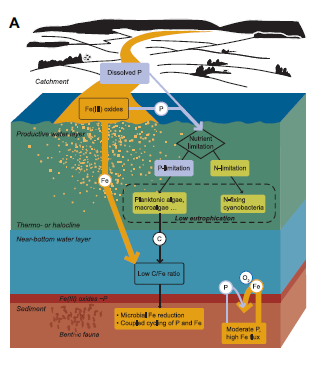
\includegraphics[width=0.8\textwidth]{../Kuvat/eutrophication_A.png}
  \caption{Expected effects of eroded soil on eutrophication on estuary in case of high amount of \ch{Fe} oxide flux \cite{Soil erosion}.}
\end{figure}

If erosion control measures takes place in the catchment of an estuary, we might see a decrease of \ch{Fe} oxides due to lowered flow of soil, but an increase in dissolved \ch{P}. The increase of \ch{P} is common outcome of reduced tilling. The increased amounts \ch{P} triggers algal production, which increases the flux of organic \ch{C} to the sediment surface. As the amount of \ch{C} increases the \ch{SO4} reduction becomes more important. The reduction in the \ch{Fe} oxide flux further promotes the importance of \ch{SO4} reduction as the \ch{C}/\ch{Fe} ratio is increased. As \ch{SO4} reduction rate increases, more of the sediment \ch{Fe} is transformed into non-sorptive \ch{Fe} sulfides. Now the "ferrous wheel" is broken and \ch{Fe} bound \ch{P} stored in sediments is released causing the estuary to be highly eutrophic. The benthic fauna of the sediment is largely gone and we might observe large cyonobacterial blooms. This state is difficult to reverse, due to the requirement of a shift in sediment microbial processes and a successful load reduction. This outline is visualized in figure \ref{fig:eutroB}.
\begin{figure}[h!]
   \label{fig:eutroB}
   \centering
   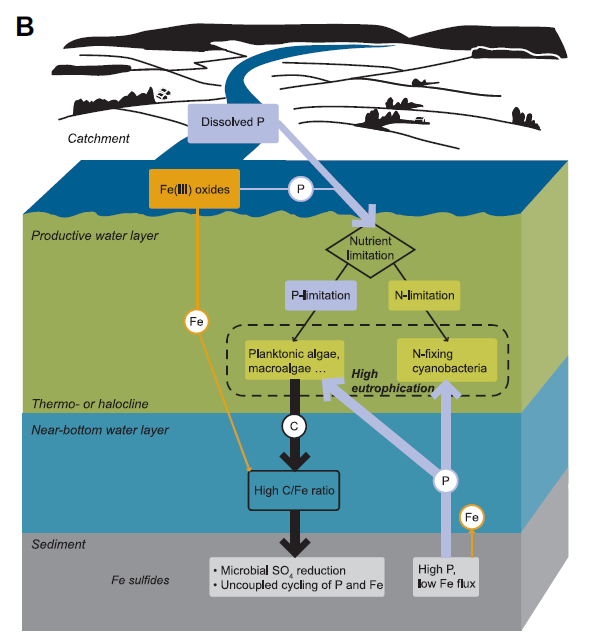
\includegraphics[width=0.8\textwidth]{../Kuvat/eutrophication_B.png}
   \caption{Expected effects of eroded soil on eutrophication on estuary in case of low \ch{Fe} oxide flux \cite{Soil erosion}}
\end{figure}

The effect of increase in \ch{C} production, caused by \ch{P}, are not straight forward. The settling flux is affected by the hydromorphology and chemistry of the receiving water body. For example in deep systems the \ch{C} is largely mineralized in water phase, and benthic processes are almost non-existent. The depth profile also affects sediment accumulation. Lastly any barriers in \ch{O2} transport to near bottom waters, such as thermocline and halocline, affect the sediment state. 

The availability of \ch{SO4} is obviously crucial for sediment processes. With low \ch{SO4} levels, the \ch{SO4} reduction plays only minor role. The \ch{P} can be expected to be desorbed in soil particles, in addition to \ch{P} in dissolved form.

If eroded soil improves the ability of the soil to preserve the \ch{P} by promoting \ch{Fe} reduction and later by coupled \ch{Fe} and \ch{P} cycling, the net effect on eutrophication depends on the balance of following factors:
\begin{enumerate}
\item Labile soil \ch{P} that can support algal primary production.
\item The lowering of benthic \ch{P} release caused by \ch{Fe} oxides.
\end{enumerate}
The balance is evidentially site-spesific, but it is possible to estimate it by determining the rate of \ch{Fe} that is available for \ch{Fe} reducing microbes and also by determining rate of dissolved \ch{P}.


\section{The Sediment as a Research Interest}
In this research we are using x-ray absorption spectroscopy to study the sediments in different environments and try to verify if we are able to see any shifts in chemical environment. We try to simulate the path of the soil by first measuring the spectra of different soil types, which have been dried and filtered. Then we are going to mix the soils with estuary waters and vary the level of labile organic \ch{C} and \ch{S}. Lastly we introduce an anaerobic environment. The absorption spectra will be measured in each case and we try to trace whether there is a shift in the chemical state or not. We are expecting the chemical state to remain similar during the two first experiments and in the third one according the outline described in section \ref{Outline}, we are expecting to see an increase of \ch{Fe} sulfides in our samples.

If our method of sediment research works, it can be applied to measure large set of different water and soil types to further study the effects of soil erosion and agriculture in different water types.

\chapter{X-ray Absorption Spectroscopy}\label{XAS}
X-ray absorption spectroscopy (XAS) focuses on studying how x-rays are absorbed above and below the element specific jumps in the absorption cross-section called absorption edges. XAS allows studying of the local structure around selected element in the sample. XAS does not require long range order, and it can be applied not only to crystals, but to amorphous systems, glasses, quasicrystals, disordered films, membranes, solutions, liquids, metalloproteins, molecular gases etc. These multiply measurement systems make XAS versatile tool in various different fields, such as physics, chemistry, biology, medicine, engineering, environmental science and geology.

X-ray absorption measurements are relatively straightforward. The main difficulty is obtaining a energy-tunable x-ray source. Traditionally this has meant synchrotron radiation sources, but lately laboratory systems based on analyzer crystals have gained some ground due to limited synchrotron beam time and due to price drop of the crystals. Many experimental techniques and sample conditions can be applied in XAS measurement, where the most limiting factors are often the energy range, beam size and intensities available from the x-ray source.  

The term "XAS", also known as "XAFS" (X-ray Absorption Fine Structure), is an upper level term for various techniques. XAS is typically divided into the XANES (X-ray Absorption Near Edge Spectroscopy) region, which focuses on the energies at vicinity of the absorption edge, and the EXAFS (Extended X-ray Absorption Fine-structure Spectroscopy), which focuses on the energies well above the absorption edge.

\section{X-ray Absorption and Fluorescence}   
In XAS measurement the basic physical quantity to measure is the x-ray absorption coefficient $\mu(E)$, which describes the probability that x-rays will be absorbed as a function of energy. Typically the $\mu(E)$ decreases smoothly as energy is increased, approximately as $1/E^3$ \cite{?}. However there are sudden jumps in the absorption cross-section at certain energies. These jumps are characteristic of the atoms in the materials and they occur when the x-ray photon has equal energy to that of the binding energy of a core-level electron, and they are called absorption edges. 

The absorption coefficient can be obtained from Beer's law:
\begin{equation}
I=I_0e^{-\mu x} \Rightarrow \mu(E)= ln{\frac{I_0}{I_x}}, 
\end{equation}
where $I_0$ is the intensity of x-rays incident on a sample, $x$ is the sample thickness and $I$ is the intensity transmitted through the sample.   
For most x-ray energies the absorption coefficient is a smooth function of energy
\begin{equation}
\mu\approx\frac{\rho Z^4}{AE^3},
\end{equation}
where $E$ is the x-ray energy, $\rho$ the sample density, $\Z$ the atomic number and $A$ the atomic mass.
\section{Theoretical Description of XAS}
X-ray absorption is a transition between two quantum states. In the initial state an x-ray, a core-electron, and no photo-electron are expected, and in the final state no x-ray, a core hole and a photo-electron. With the initial and final state we can describe the $\mu(E)$ with Fermi's Golden Rule

\begin{equation} \label{eq:Fermi}
\mu(E) \propto |\braket{i | H | f}|^2
\end{equation}

where $\bra{i}$ is the initial state, and the $\ket{f}$ the final state, and $H$ is the Hamiltonian representing the interaction. The core-electron is tightly bound in the absorbing atom, so the initial state is not altered in the presence of a neighbouring atom. However the photo-electron will be able to see the neighbouring atom and thus the final state will be affected. By expanding the $\ket{f}$ into two pieces, $\ket{f_0}$ that represents the bare atom portion and the $\ket{\Delta f}$ represents the neighbouring atom, we get  

\begin{figure}[h!]
  \label{fig:free atom}
  \centering
  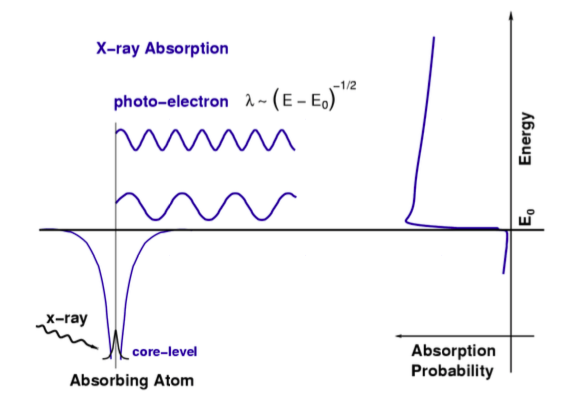
\includegraphics[width=0.8\textwidth]{../Kuvat/absorption1.png}
  \caption{The x-ray absorption through the photoelectric process is expressed visually above. When the incident photon has the energy of a tightly bound electron level, $E_0$, the absorption probability has a clear edge. The tightly bound core level is destroyed in the process and a photo-electron is created. The photo-electron travels as a wave with wave number proportional to $\sqrt{(E-E_0)}$} \cite{?}.
\end{figure}

\begin{equation}
\ket{f}=\ket{f_0}+\ket{\Delta f} 
\end{equation}
which can be applied to equation \ref{eq:Fermi}
\begin{equation}
\mu(E)\propto |\braket{i | H | f}^2[1+\braket{i|H|\Delta f}\frac{\braket{f_0|H|i}^*}{|\braket{i|H|f_0}|}+C.C]
\end{equation}
where $C.C.$ stands for complex conjugate. This resembles the closely previously discussed relation between $\mu(E)$ and $\chi(E)$  
\begin{equation}
\mu(E)=\mu_0(E)[1+\chi(E)].
\end{equation}

\begin{figure}[h!]
  \label{fig:neighbour atom}
  \centering
  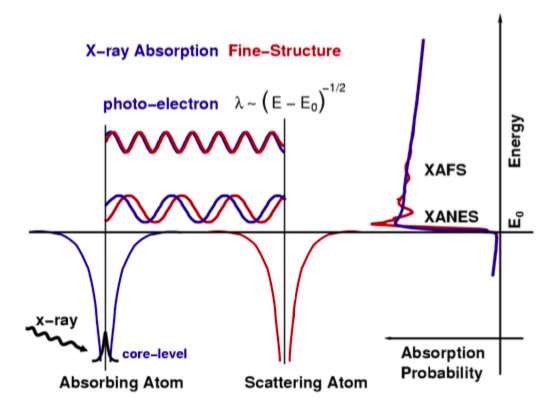
\includegraphics[width=0.8\textwidth]{../Kuvat/absorption2.png}
  \caption{something}
\end{figure}
Combining the previous equation allows us to assign $\mu_0=|\braket{i|H|f_0}|^2$ as the bare atom absorption, which depends only on the absorbing atom. We also note that the fine-structure $\chi$ can be written as
\begin{equation}
\chi(E)\propto\braket{i|H|\Delta f}.
\end{equation}
\section{Transmission}
\section{The XANES Section of the Spectrum}
The XANES region is much easier to measure than the EXAFS region. This is mainly due to the fact that the intensity oscillations are larger and the energy range is smaller. XANES can be done with lower concentrations and the restrictions in sample conditions are not as tight. However the XANES cannot be simply solved analytically, since the EXAFS equation breaks down at low $k$ values, mainly due to the $1/k$ term and the increase in mean-free-path at very low $k$. This however doesn't mean that we couldn't draw any conclusion from the spectra, since there is much chemical information in the XANES region. Most notably the 

\subsection{Oxidation Number}
The absorption edge is loosely defined. Typically it is defined as half height of the edge or as maximum of the first derivative with respect to energy. Often the definition is not as straight forward, since the edge spectra might have unresolved transitions superimposing on the rising edge. These make the definition of a unique edge energy rather troublesome. Even though the definition can be ambiguous, the edge energies are useful tool for determination of oxidation state of the absorber. The energy of an edge increases as oxidation state of the absorber increases. By using electrostatic model we can note that atoms with higher oxidation state should have higher charge, and to eject a core electron, a higher energy x-rays are needed. 

\begin{figure}[h!]
\label{fig:XANESfetures}
  \centering
  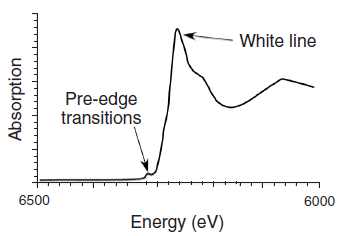
\includegraphics[scale=0.8]{../Kuvat/XANESfeatures.png}
  \caption{Figure showing different features in the XANES region \cite{?}.}
\end{figure}

Alternatively we can treat the edge features as "continuum resonances". A continuum resonance involves excitation of a core electron into a high-energy state, above the continuum, with a finite lifetime. Let's use the potential well between absorbing and scattering atoms as an example. As the distance between the atoms gets shorter, the energy of the continuum state increases as $1/R^2$. Higher-oxidation-state metals have shorter bond lengths this model also predicts the increase in edge energetic with increasing oxidation state. The remark of higher oxidation number increasing the edge energy is widely used in coordination chemistry.

\begin{figure}[h!]
\label{fig:FeOxidation}
  \centering
  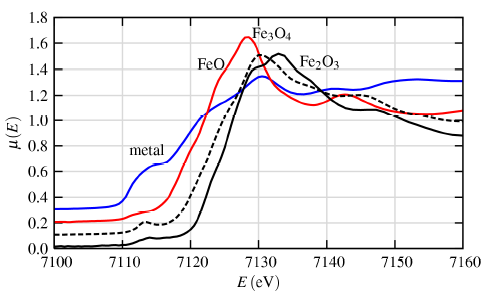
\includegraphics[scale=0.8]{../Kuvat/FeOxidation.png}
  \caption{\ch{Fe} $K$-edge XANES spectra of metallic \ch{Fe} and some \ch{Fe} oxides. The graph clearly shows relation between oxidation state and edge energy \cite{Fundamentals}.}
\end{figure} 

The figure \ref{fig:FeOxidation} is a great example of the valance dependence of the metallic \ch{Fe} and other \ch{Fe} oxides. With good quality reference samples it is easy determine the ratios of different oxides in the sample.      

\subsection{Multiple Scattering Events}
The x-ray excited photoelectron can be scattered by more atoms than a single one. In fact photoelectron can scattered by two or more atoms prior to returning to the absorbing atom, as seen in figure \ref{fig:ms}. The XANES region is sensitive to multiple scattering events, since the the photoelectron has a low kinetic energy and the mean free path is increased. In addition the Debye-Waller damping factor is $\exp{-k^2}$ dependent and thus negligible in the XANES region. Multiple scattering events complicates simulation of XANES, since there are more interactions and large number of multiple scattering pathways. Even though the multiple scattering events complicates simulations, they also provide a possibility to extract information about the three-dimensional structure from XANES spectra \cite{?}. Recently the simulations have become more and more accurate \cite{?}, but most of the simulations still remain qualitative.

\begin{figure}[h!]
\label{fig:ms}
  \centering
  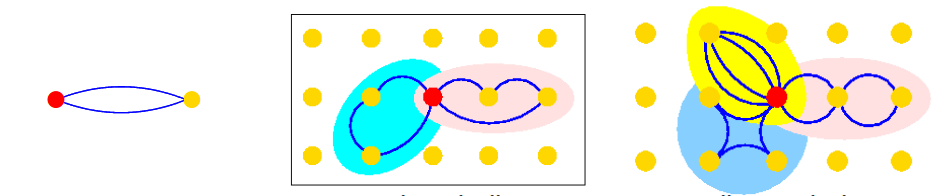
\includegraphics[scale=1]{../Kuvat/multiplescattering.png}
  \caption{Dashed line represents single scattering, and solid lines multiple scattering pathways. $A$ is the absorbing atom, which in this example is surrounded by two scattering atoms, $S_1$ and $S_2$ \cite{?}.}
\end{figure}

The changes in the three-dimensional structure can be seen empirically in the XANES spectra. Even small variations in structure can be seen in spectra, and for example two sites with identical EXAFS spectra can have distinct XANES spectra. Geometrical differences between sites alter the multiple scattering pathways, and this atleast partly explains the site sensitivity of XANES. The interpretation of XANES spectra has been progressing steadily, but the agreement between computational and observed spectra remains quite poor in most cases. The development of theoretical and computational model for detailed interpretation of XANES spectra remains one of the main challenges in the field.         

\subsection{Bound States Transitions}
In the figure \ref{fig:XANESfetures} we see a weak pre-edge peak. The pre-edge peak is caused by bound state transitions. In case of K edge of a first row transition metal, the peak is caused by $1s\rightarrow 3d$ transition. The $1s\rightarrow 3d$ transition is not allowed transition according to dipole selection rule, but it is still observed due to $3d+4p$ mixing and to direct quadrupolar coupling.   
\subsection{Multi-electron Transitions}

\chapter{HelXAS}\label{setup}
\section{Setup}
The HelXAS equipment was built by the X-ray Laboratory staff. The instrument is based around three basic components: x-ray tube, monochromator and scintillator counter (detector). The monochromator crystal is placed on a motorized rail, and it can also be rotated around its vertical axis essentially to change the angle of the monochromated beam. The detector is also placed on two motorized rails to allow the movement in two dimensions. The x-ray tube is fixed in position. These components follow the so called Rowland circle geometry. Rowland circle is a Bragg reflection geometry, which allows simultaneous focusing and energy analysis of the fluorescence source. The setup is shown in figure  The movements and data collection is done by using Spec 6 software, which a specialized software for x-ray spectroscopy \cite{?}.

\begin{figure}[h!]
  \centering
  \label{fig:setup}
  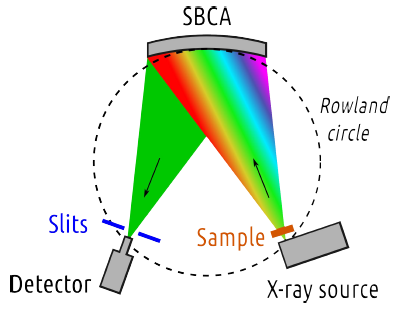
\includegraphics[width=0.8\textwidth]{../Kuvat/helxasSetup.png}
  \caption{Illustration of the measurement setup.}
\end{figure}
\subsection{X-ray Source}
HelXAS is designed to measure 3d transition metal K edges in the energy range $\approx 5-15 \si{\kilo\electronvolt}$. The x-ray tube in the setup uses silver anode, since \ch{Ag} has characteristic lines above $20\si{\kilo\electronvolt}$ \cite{}.     
\subsection{Monochromators}
The X-rays spectra produced by the X-ray tube is polychromatic and is thus not very useful for our purpose to vary the energy in a small energy band. To make the x-ray beam more useful we use a monochromator crystal. The crystal is used for point-to-point scanning, where a small energy bandwidth ($<5\si{\electronvolt}$) satisfies Bragg's diffraction condition over the whole crystal area and is focused on the detector \cite{Analyzer crystal}. The Bragg's diffraction condition 
\begin{equation} \label{eq:bragg}
2d_{hkl}\sin\theta_b=n\lambda,
\end{equation}
where $d_{hkl}$ is the distance between atoms in a lattice, $n$ is an integer, $\theta_b$ theta the angle between incident beam and diffracted beam and $\lambda$ is the wavelength of the diffracted beam. The distance $d_{hkl}$ is proportional to the miller indices, and by selecting the right crystal orientation we can also selected the wanted energy bandwidth in a point-to-point measurement. The wavelength is related to energy by 
\begin{equation}
\lambda=\frac{hc}{E},
\end{equation} 
where $h$ is Planck's constant and $c$ speed of light in a vacuum. 

For our measurement we use an analyzer crystal with miller indices $hkl=[3,5,1]$, which allows us to scan the around the k-absorption edge of \ch{Fe} at $E=7.1 \si{\kilo\electronvolt}$, by varying the angle $\theta$.

The analyzer crystal is bent

\subsection{Scintillator Detector}
The setup uses doped \ch{NaI} crystal, which converts the x-ray photons to low energy photons, which are converted to a cascade of electrons. These pulses are collected and transformed into voltage pulses. Pulses are proportional to photon energy, but the energy resolution is poor.

The detector has a finite response time to incident photons, known as dead time $\tau$. During that time the detector cannot count other photons. For sufficiently small dead time we can use the following correction

\begin{equation} \label{eq:deadtime}
N_{correct}\approx\frac{N}{1-\frac{\tau}{T}N},
\end{equation}
where $N$ is the number of counted pulses and $T$ is the time in which they were acquired.

\subsection{Preparations for Anaerobic Samples}
For the anaerobic samples we had to design a new sample environment. In our design the sample is placed between two $0.1 \si{\milli\metre}$ kapton foils, and sealed with $1 \si{\milli\metre}$ thick o-ring. This setup is compressed by two aluminium plates and eight screws. The window on the aluminium plates has a diameter of $10 \si{\milli\metre}$, and there are 8 slots for samples. The design is show in figure \ref{fig:n�ytteenvaihtaja}.

\begin{figure}[h!]
  \label{fig:n�ytteenvaihtaja}
  \centering
  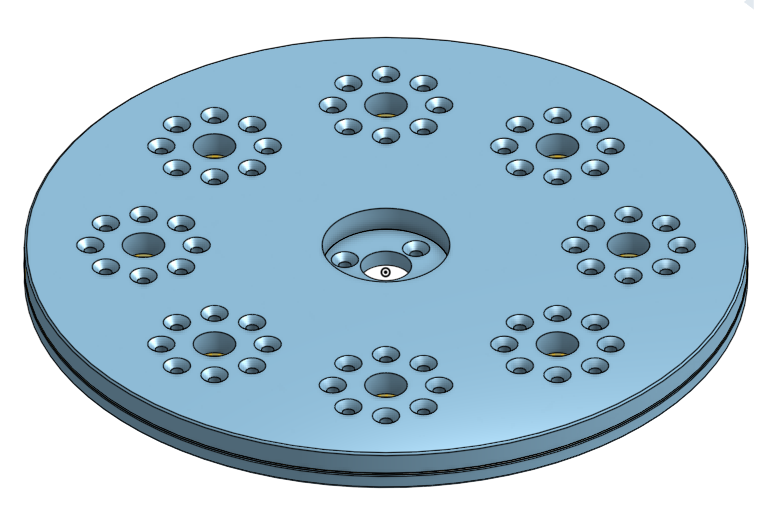
\includegraphics[width=0.8\textwidth]{../Kuvat/vaihtaja.png}
  \caption{The design of the anaerobic chambers.}
\end{figure}
The sample plate is motorized, which allows us to automate the measurements.

\subsection{Background Noise}
When doing the measurement, the background noise is always present. Background noise is caused by elastic scattering, fluorescence, etc. Since the $\mu x$ is obtained from a logarithm, it is highly non-linear, and thus sensitive to background noise. 

The background noise can be taken into account by measuring it by moving the detector away from the direct beam. The accuracy of background measurement can be improved by measuring the background from both sides of the beam and taking the mean. The background is slowly varying, so in order to avoid statistical noise, a low order polynomial is fitted and the fit is removed from the signal.    

\subsection{Measurement Procedure}
First we measure the direct beam $I_0$ and the transmitted beam $I$ and their backgrounds $I_{0,bg}$ and $I_{bg}$. Then we apply the dead time correction from equation \ref{eq:deadtime}. Next we fit low order polynomials $y$ and $y_0$ to the backgrounds $I_{0,bg}$ and $I_{bg}$. Finally we compute the $\mu x$ from equation

\begin{equation} \label{eq:mux}
\mu  x=\ln\frac{I_0-y_0}{I-y}.
\end{equation}


\chapter{Sample Preparation}\label{preparation}
\section{Reference Samples}\label{ref}
In order to estimate the chemical state of our system, we acquired a set of reference samples of some well known iron compounds. These samples can be used as a fingerprint for each compound and allow us keep track of the chemical state of our soil samples. In all of our  measurements we used $0.01\si{\milli\metre}$ iron foil to keep track of our energy calibration. 
\section{Samples}\label{samples}
\subsection{Soil Samples}
The soil we received was obtained from five different locations. The soil was weighted by using a scale with an accuracy of $10^{-4} \si{gram}$. The soil was then mixed with farina in approximately 1:4 concentration. After mixing we added some ethanol and ground using a mortar until the ethanol was evaporated. The result was a fine mix with a uniformly small particles. The mix was then placed in a M5 washer and was sealed with Scotch tape. From the five different soils we made two samples of each.  
\subsection{Slurries}
The measurement of wet samples turned out to be trickier than expected. When the sample was placed in front of the X-ray tube, the bremsstrahlung caused by the x-ray and sample atom interaction, broke the bonds in the water molecules. The broken water molecules released \ch{O}-radicals, which interacted with our samples and after few ours all the water in the sample was gone, and the chemical state of the sample was altered.

Second problem we encountered was the sample homogeneity. When the soil is mixed with water, it tends to sediment. The sedimentation causes soil to accumulate at the bottom of the sample environment. Also when the sample is rotated, the smaller particles move faster and larger particles/clusters may stay still. Now when if place the sample in front of the detector and scan the energy range by changing the angle $\theta$, we might hit just the water or the soil with different thickness or particle size. 

In order to tackle the problems stated above we decided to gel our samples with agar. We took the water where the samples were mixed in, and added approximately $1-0.5wt\%$ of agar. The water was then heated to boiling and mixed all the time with magnetic stirrer. Heating was turned off when the water reached boiling temperature and the sediment was mixed with water after the water reached approximately $60\si{celcius}$. The mix was then quickly placed in the sample environment and cooled in a fridge. This method allowed us to make homogeneous samples to be placed in front of the detector. 

We tested the optimal water/soil ratio for our samples by mixing soil and water in ratios 1:4, 1:8 and 1:16. We then measured the absorption spectra of these mixes and the results are shown in figure \ref{fig:jellytest}.
\begin{figure}[h!]
   \label{fig:jellytest}
   \centering
   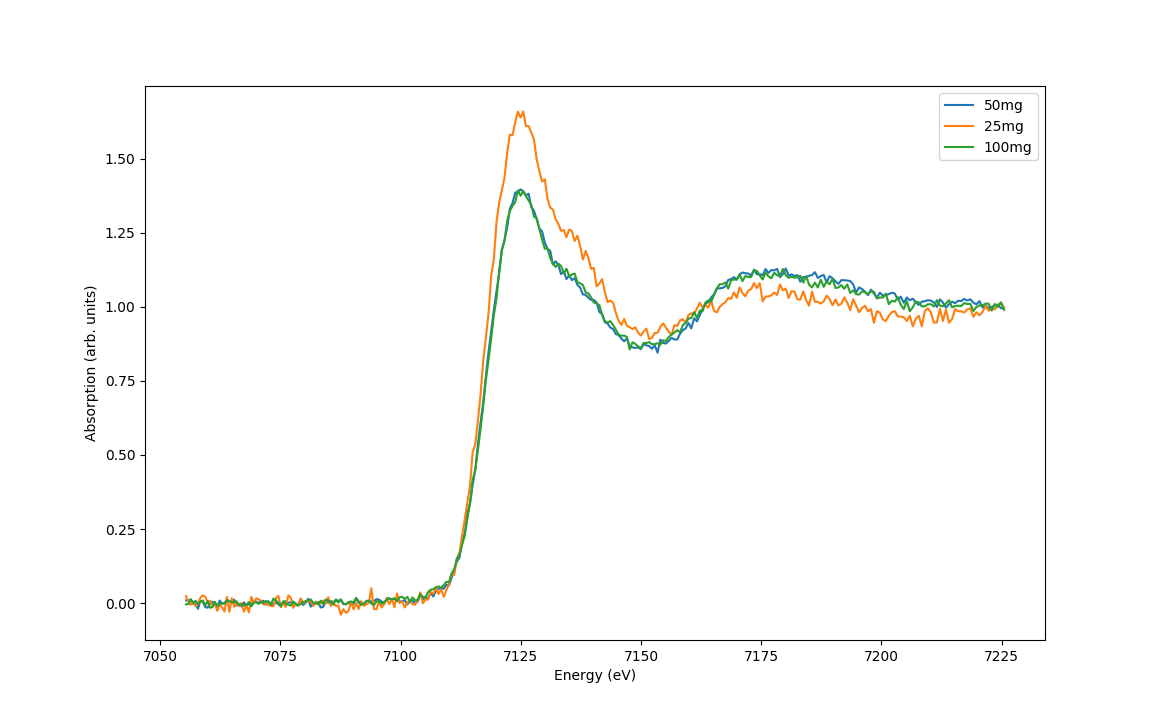
\includegraphics[width=\textwidth]{../Kuvat/JellyTest.png}
   \caption{The x-ray absorption spectra different gel mixes.}
\end{figure}
As a result for this test we concluded that we need high enough soil/water concentration to make the normalization of our spectra easier. 
\subsection{Anaerobic Slurries}
The sample preparation of anaerobic wet samples was rather similar to the preparation of our normal wet samples. The major difference was that the sample preparation was done in \ch{N} atmosphere. 

\subsection{The Affects of Agar}


\chapter{Results and Analysis}\label{tulokset}
\section{Analysis}
\subsection{Data Reduction}
We used following steps to reduce our data:
\begin{enumerate}
\item The measured intensities are converted to $\mu(E)$.
\item A smooth line is fitted to the pre-edge region of the spectrum and then subtracted from the $\mu(E)$ in order to get rid of the instrumental background and absorption from other edges.
\item The threshold energy $E_0$ is identified as the maximum derivative of $\mu(E)$.
\item $\mu(E)$ is normalized from 0 to 1, so that it represents the absorption of 1 x-ray.
\end{enumerate}
\subsection{Interpretation of the XANES-spectrum}
The XANES-spectrum is much larger signal than 
\subsubsection{Oxidation Number}
The threshold energy of the absorption edge is loosely defined. Most commonly it is defined as maximum derivative of the $\mu(E)$, or as half of the height of the edge. The absorption spectrum might have multiple 
\subsubsection{Multiple Scattering Events}
\subsubsection{Binding Energy Shifts}
\section{Measurement results}
\subsection{Soil Samples}
All the soil samples had a relatively similar spectra
\begin{figure}[h!]
  \label{fig:drySoil}
  \centering
    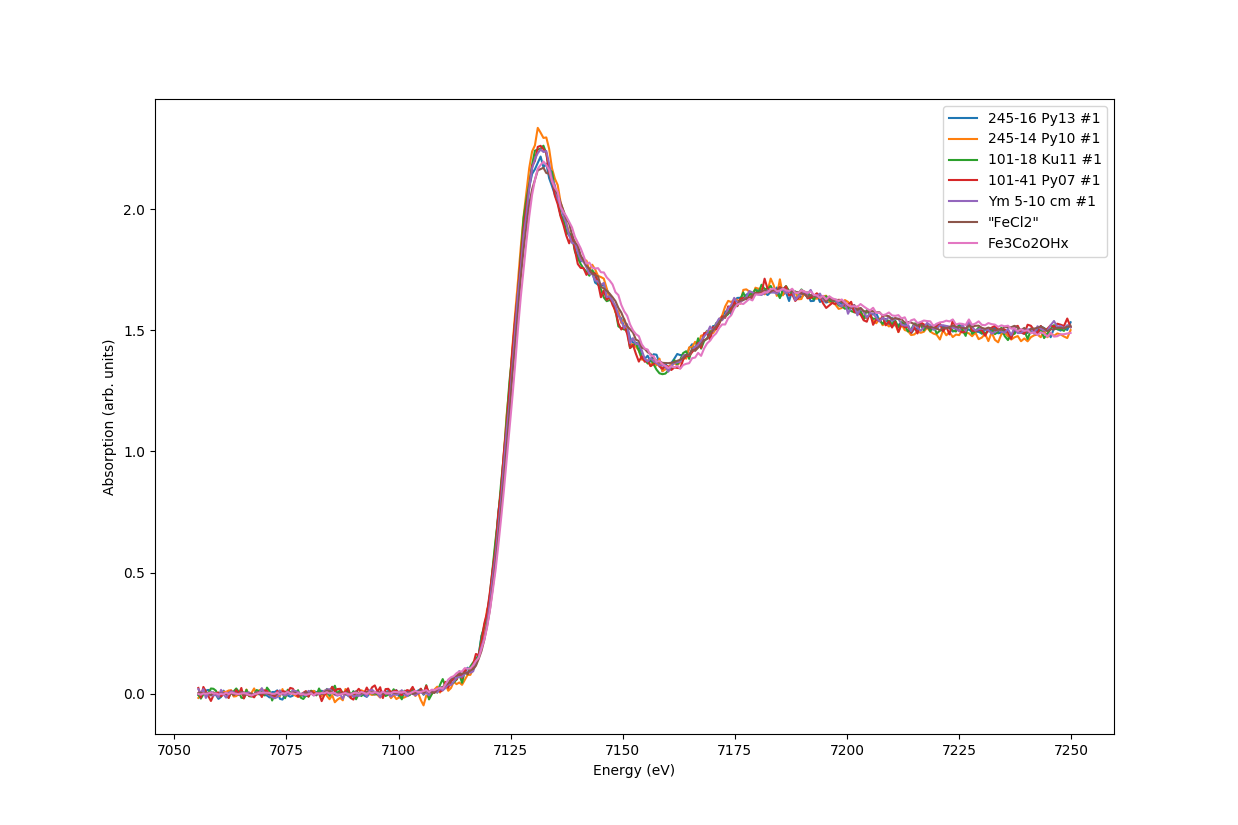
\includegraphics[width=\textwidth]{../Kuvat/Dry_Soil_Samples1.png}
  \caption{The spectra of dry soils.}
\end{figure}

\begin{figure}[h!]
  \label{fig:dryHomogenity}
  \centering
    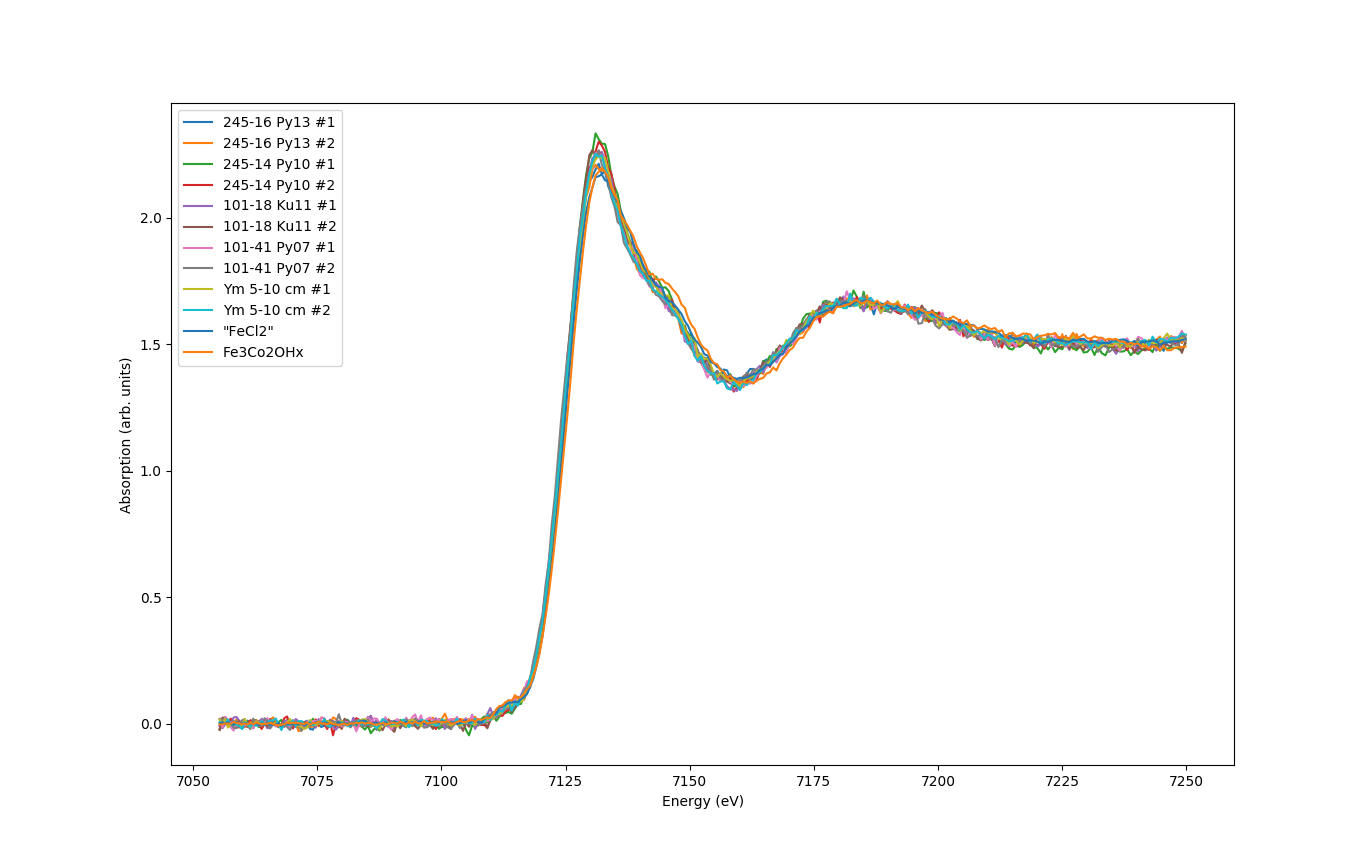
\includegraphics[width=\textwidth]{../Kuvat/dry_soil_samples_all.png}
  \caption{The spectra of all dry soils.}
\end{figure}
\subsection{Slurries}
\subsection{Anaerobic Slurries}

\chapter{Conclusion}\label{conc}



\begin{thebibliography}{9}

\bibitem{Fe concentration}
Chesworth W.
\textit{Geochemistry of micronutrients} In. Mortvedt, J.J., Cox, F.R., Shuman, L.M., Welch, R.M. (Eds.), \textit{Micronutriens in Agriculture}, Soil Science Society of America, Inc., Madison, Wisconsin, USA, pp. 1-30.

\bibitem{Soil erosion}
Petri Ekholm, Jouni Lehtoranta.
\textit{Does control of soil erosion inhibit aquatic eutrophication}.
Journal of Environmental Management 93 (2012) 140-146.

\bibitem{Labile carbon}
Lehtoranta J., Ekholm P., Wahlstr�m S., Tallberg P., Uusitalo R.
\textit{Labile organic carbon regulates phosphorus release from eroded soil transported into anaerobic coastal system}.
Ambio 2015, 44(Suppl. 2) 263-273.

\bibitem{Ros}
Jilbert T., Asmala E., Schr�der C., Tiihonen R., Myllykangas J-P., Virtasalo J. J., Kotilainen A., Peltola P., Ekholm P., Hietanen S.
\textit{Impacts of flocculation on the distribution and diagenesis of iron in boreal estuarine sediments}.
Biogeosciences 15 (2018) 1243-1271. 

\bibitem{Elements}
Elements of Modern X-ray Physics, J. Als-Nielsen and D.McMorrow, John Wiley \& Sons, 2001.

\bibitem{Analyzer crystal}
Rovezzi M., Lapras C., Manceau A., Glatzel P., Verbeni R.
\textit{High energy-resolution x-ray spectroscopy at ultra-high dilution with spherically bent crystal analyzers of 0.5 m radius}.
Rev.Sci.Instrum.88 (2017) no.1

\bibitem{Optic alignment}
Mortensen D., Seilder G.
\textit{Robust optic alignment in a tilt-free implementation of Rowland circle spectrometer}.
Journal of Electron Spectroscopy and Related Phenomena, Volume 215, February 2017, Pages 8-15

\bibitem{Fundamentals}
Fundamentals of XAFS, Matthew Newville \url{https://web.archive.org/web/20110722032112/http://xafs.org/Tutorials?action=AttachFile&do=view&target=Newville_xas_fundamentals.pdf}

\bibitem{Tuo}
Pekka Tuominen: Todenn�k�isyyslaskenta I, 5.\ painos, Limes ry, 2000.

\end{thebibliography}

\end{document}
